\documentclass[13pt,journal,draftclsnofoot,onecolumn]{IEEEtran}

\usepackage{latexsym}
\usepackage{amssymb}
\usepackage{amsbsy}
\usepackage{amsmath}
\usepackage{multirow}
\usepackage{listings}
\usepackage{xcolor}

\lstset{ %numbers=left,
	%numberstyle= \tiny,
	basicstyle=\ttfamily\scriptsize,
	keywordstyle=\color{blue}\ttfamily,
	stringstyle=\color{red}\ttfamily,
	commentstyle=\color{green}\ttfamily,
	breaklines=true,
	showstringspaces=false,
	keepspaces=false,
	frame=shadowbox,
	extendedchars=false,
	tabsize=4,
	showspaces=false
	%rulesepcolor= \color{ red!20!green!20!blue!20}
}

\usepackage{longtable}
\usepackage{pifont}
\usepackage{times}
\usepackage{graphicx}
\usepackage{subfigure}
\pagestyle{plain}


\newcommand{\rmv}[1]{}
%\renewcommand{\baselinestretch}{1.6}
%\renewcommand{\thesection}{\Roman{section}.}
%\renewcommand{\thesection}{\arabic{section}}
%\renewcommand{\thesubsection}{\Alph{subsection}.}
%\renewcommand{\thesubsection}{\arabic{section}.\arabic{subsection}.}
%\renewcommand{\theequation}{\arabic{equation}}
%%\renewcommand{\theequation}{\arabic{section}.\arabic{equation}}
%\renewcommand{\thefigure}{\arabic{figure}}
%\renewcommand{\thetable}{\arabic{table}}
%\renewcommand{\thempfootnote}{\alph{footnote}}
%\renewcommand{\thempfootnote}{\fnsymbol{footnote}}

\newtheorem{theorem}{Theorem}
%\newtheorem{corollary}{Corollary}
\newtheorem{algorithm}{Algorithm}
%\newtheorem{definition}{Definition}
%\newtheorem{evaluation}{Evaluation}
\newtheorem{lemma}{Lemma}
\newtheorem{example}{Example}
\newtheorem{fact}{Fact}
%\newtheorem{property}{Property}

%\setcounter{page}{100}
\usepackage{url}
\usepackage{shorttoc}
\usepackage{color}


\usepackage{fancyhdr}
 
\pagestyle{fancy}
\fancyhf{}
\rhead{\scriptsize{\thepage}}
\lhead{\scriptsize{EE5414 Development and Design in Embedded Systems}}
\rfoot{\scriptsize{CityU EE Dept.}}
\renewcommand{\headrulewidth}{0.4pt} 
\renewcommand{\footrulewidth}{0.4pt}

\begin{document}

%\mainmatter

\baselineskip=22 pt

\begin{titlepage}

\begin{center}


% Upper part of the page

\includegraphics[width=0.15\textwidth]{./figs/logo.png}\\[1cm]    

\textsc{\LARGE City University of Hong Kong}\\[1.5cm]

\textsc{\Large Department  of Electronic Engineering}\\[0.5cm]


% Title
\rule{0.9\textwidth}{1pt}\\[0.4cm]
{ \huge \bfseries EE5414 Laboratory - Part II Report}\\[0.4cm]
\rule{0.9\textwidth}{1pt}\\[1.5cm]


% Author and supervisor
\begin{minipage}[t]{0.4\textwidth}
\begin{flushleft} \large
\emph{Author:}\\
Wangchen \textsc{DAI} (53623708)\\
Jingwei \textsc{HU} (53656463)\\
\end{flushleft}
\end{minipage}
\begin{minipage}[t]{0.4\textwidth}
\begin{flushright} \large
\emph{Instructor:} \\
Dr.~L.L.\textsc{CHENG}  
\end{flushright}
\end{minipage}

\vfill

% Bottom of the page
{\large \today}

\end{center}

\end{titlepage}

\clearpage

\section{Android Source Code compilation and Android Booting Procedure}\label{Intro}
An embedded system is a computer system with a specific function and embedded in a mechanical or electrical system. Due to the limitation of processing resources, lower power consumption, smaller size, lower cost, and simpler operating function are the main properties of embedded computers when compared with the general ones. Embedded systems are usually based on microcontrollers or microprocessors, such as MCU, ARM, DSP and FPGA. In this project, an ARM based circuit board, BeagleBone Black (BBB), is applied as the hardware development tool. Ubuntu Trusty 14.04, which is known as a version of open source Linux system, is loaded into the ARM chip as the software development platform. Using this specified embedded system, a series of functions are developed including: LED Test, Image/Video Capture, Web Server and SQL Server Establishment.


% % % % % % % % % % % % % % % % % % % % % % % % % % % % % % % % %
% % % % % % % % % % % % % % % % % % % % % % % % % % % % % % % % %
\section{Install and uninstall applications}\label{HdDes}

BBB is a low-cost, community-supported hardware device for embedded application development. BBB board mainly contains an ARM Cortex A8 series processor, a 512MB DDR3 RAM memory, an onboard 2GB MMC chip, with some other necessary peripherals. In this project, the BBB board is developed with following cables and devices: 
\begin{itemize}
\item A MiniUSB Cable, which can be used to connect the board with PC and served as power source (limited to 500mA), network, and serial port for data transmission;
\item An external DC power supply with 5V and a minimum of 1A current output;
\item A USB Hub to expand the onboard USB Host port from one to four;
\item A USB portable 802.11N wireless adapter;
\item A Logitech HD Pro C920 Web Camera, which is a USB webcam and provides full HD 1080p video recording in wide-screen at a maximum rate of 30 frames per second;
\item A mini SD card and its corresponding USB portable card reader.
\end{itemize}
The detailed and connection information of all hardware cables and devices is provided in both Fig.\ref{hw1}, for block diagram view, and Fig.\ref{hw2} for real view.
\begin{figure}[ht]
	\centering
	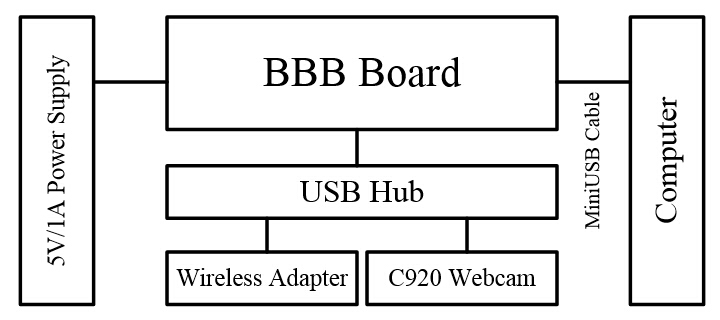
\includegraphics[width=4in]{./figs/hw1.jpg}
	\caption{Block Diagram of Hardware Description.}
	\label{hw1}
\end{figure}
\begin{figure}[ht]
	\centering
	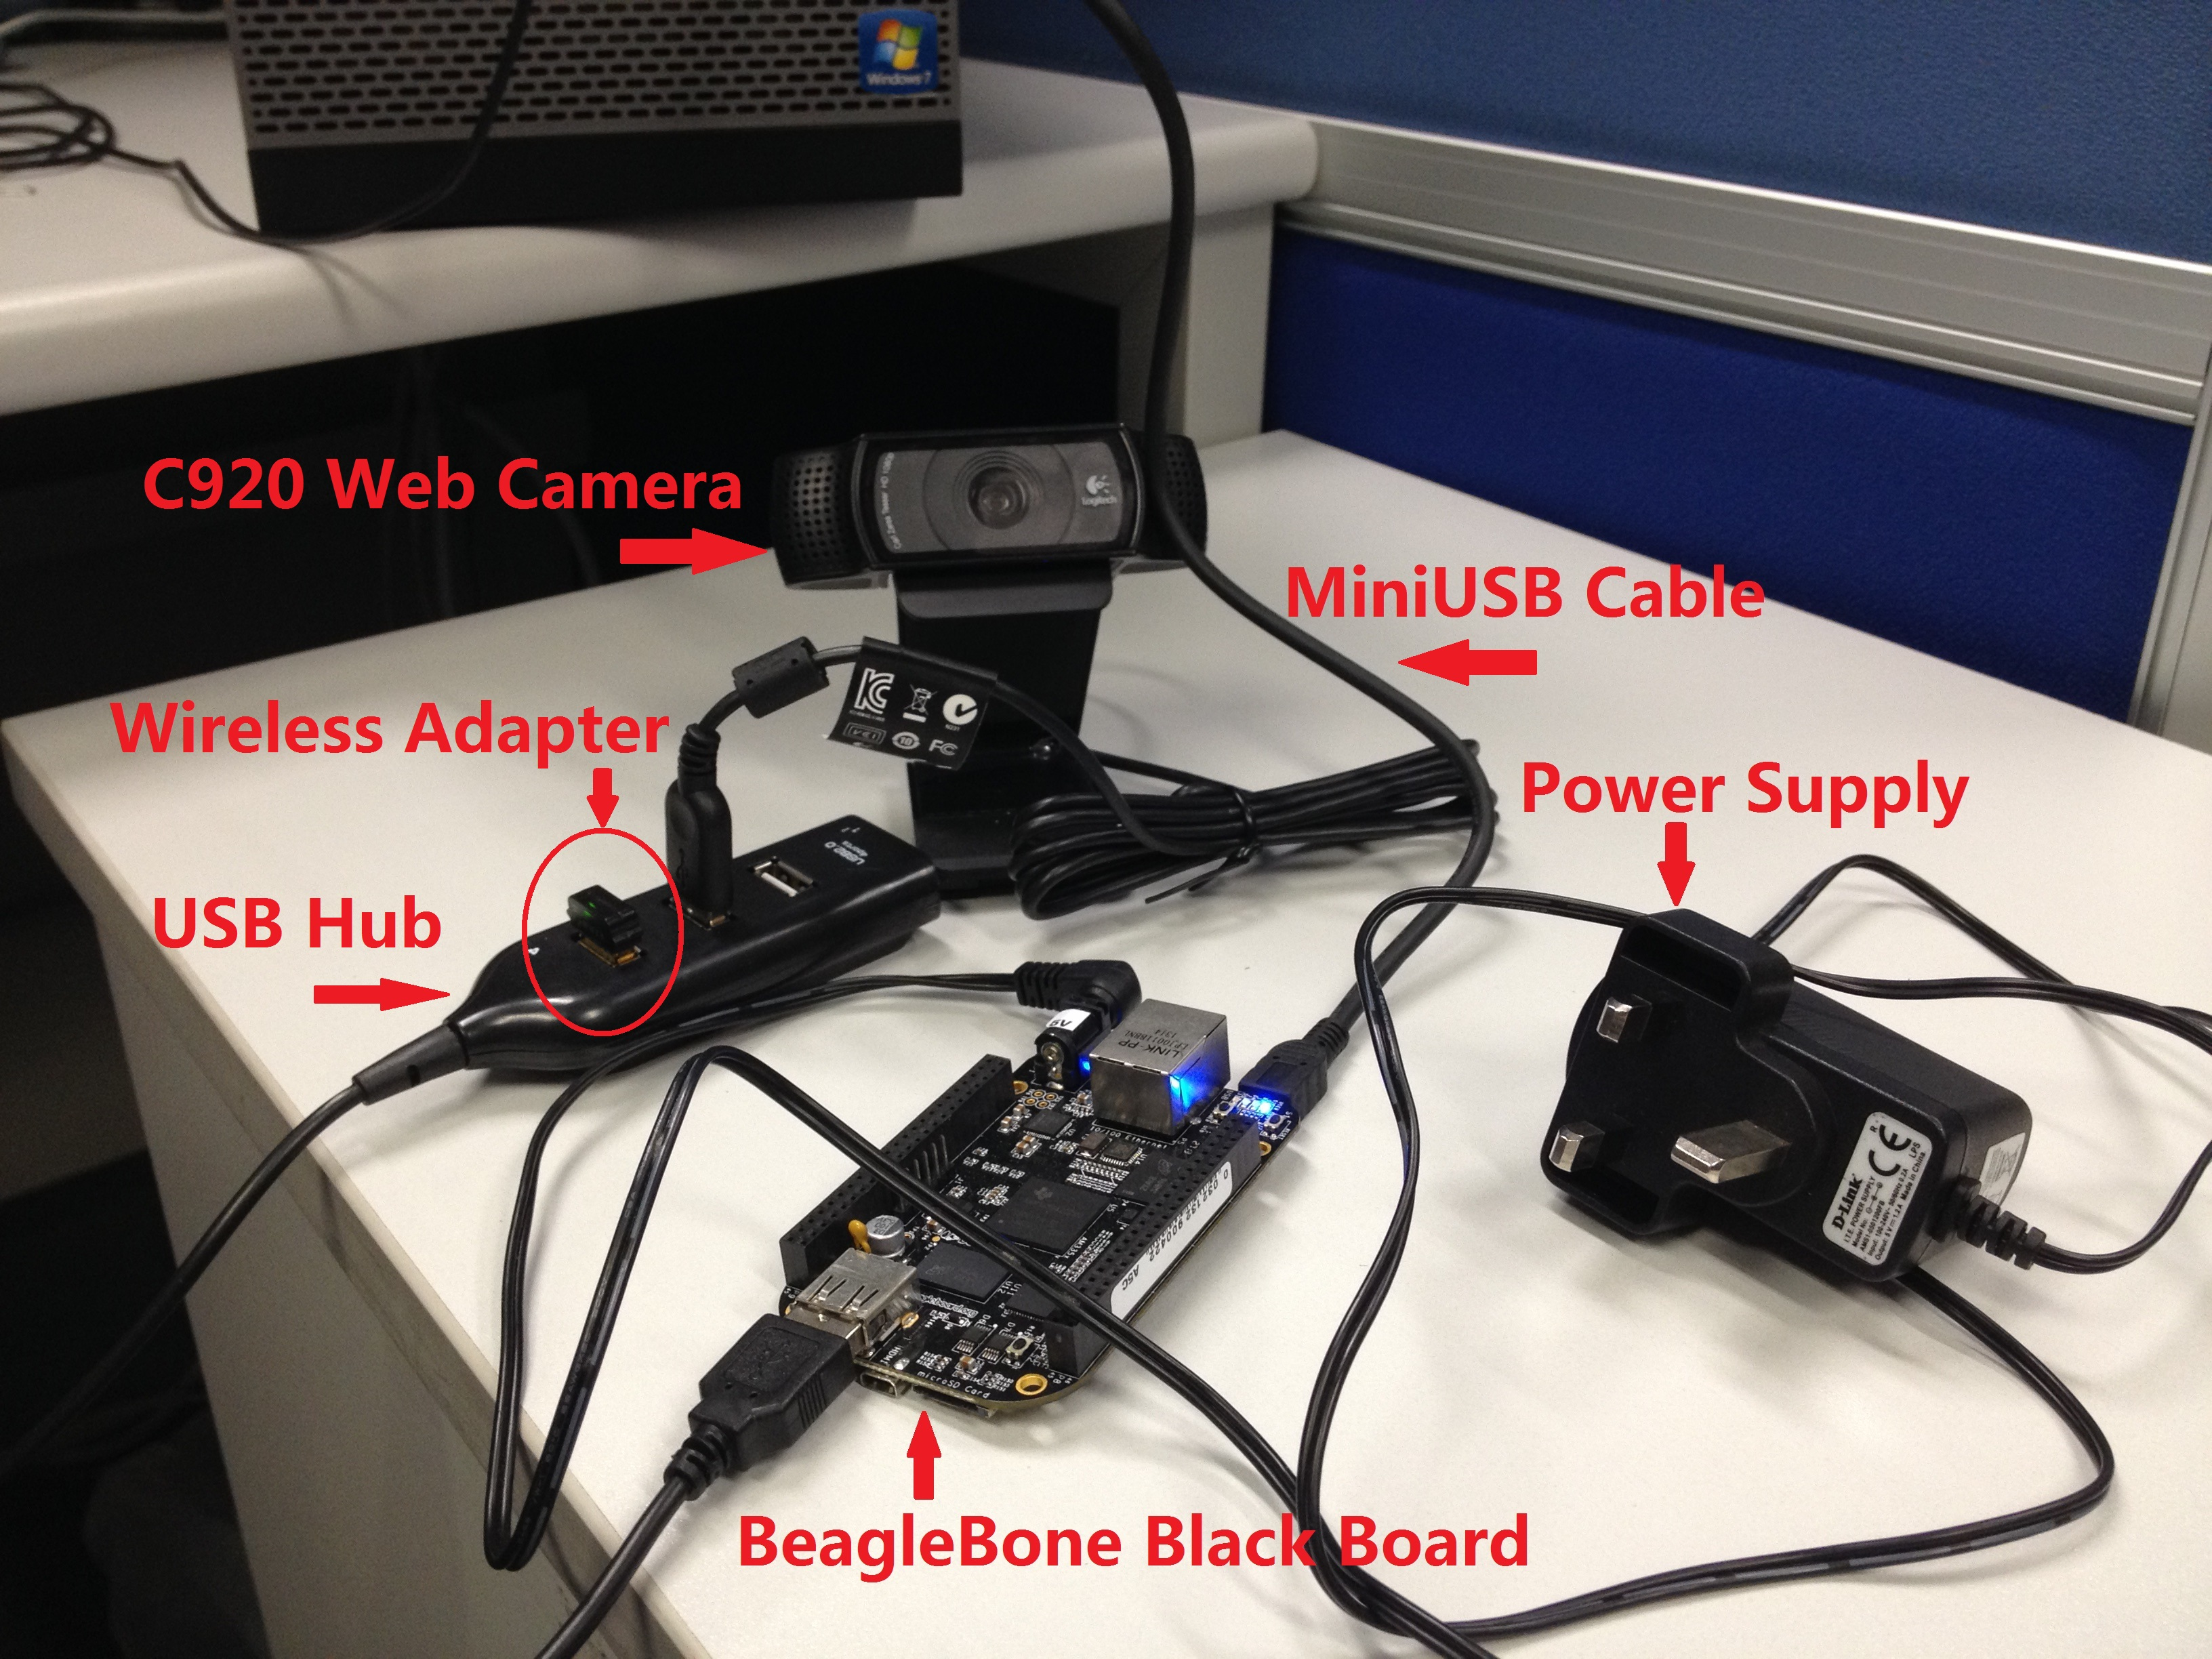
\includegraphics[width=4in]{./figs/hw2.jpg}
	\caption{Real View of Hardware Description.}
	\label{hw2}
\end{figure}

Both of the figures indicate the hardware setup details. First, the BBB board is connected to a PC using the MiniUSB Cable. Via the cable, the BBB board could not only receive a 5V/500mA power supply provided by PC's USB port, but also be accessible from a host PC and share the Internet connection by setting up Windows ICS \cite{windowsICS}; In addition, users could operate Linux instructions through specific Windows-based software clients. Second, in case of unexpected system shutdown issue caused by current exceeding (current supply using MiniUSB Cable is set at a maximum of 500mA), an external power supply is used. Third, a USB Hub is connected to the onboard host USB port for expanding the port from one to four. Finally, the Logitech C920 webcam is connected to the USB Hub with its attached USB cable, together with a USB portable wireless adapter. Note that in this project, system could have two different IP addresses for Ethernet and wireless connection, respectively, also the BBB board could have an alternative way to access the Internet: getting access to a WiFi or Hotspot connection via the wireless adapter.


% % % % % % % % % % % % % % % % % % % % % % % % % % % % % % % % %
% % % % % % % % % % % % % % % % % % % % % % % % % % % % % % % % %
\section{Running Applications}\label{SfDes}
\begin{figure}[ht]
	\centering
	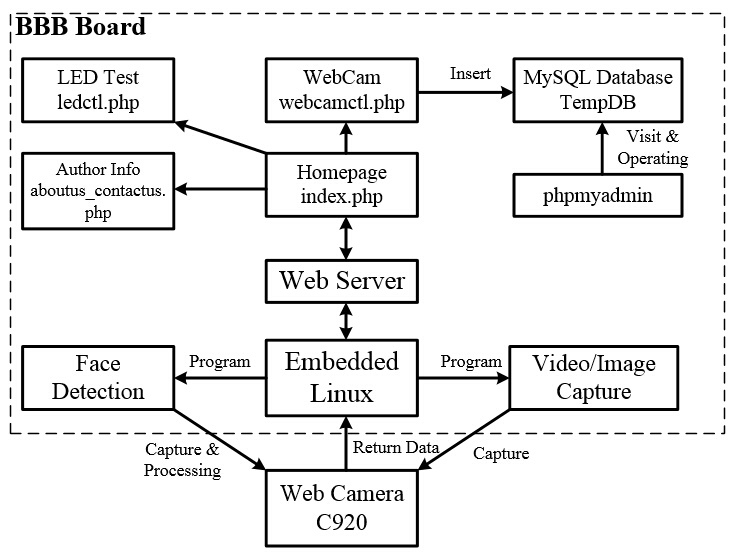
\includegraphics[width=5in]{./figs/sw1.jpg}
	\caption{Block Diagram of Software Description.}
	\label{sw1}
\end{figure}

In this project, the software implementation includes installation, configuration as well as application of embedded OS, Web server, PHP, and MySQL; setup and website-based control of onboard LEDs and the C920 Web Camera. Fig.\ref{sw1} provides a block diagram of software description.
	
\subsection{Wireless Adapter Configuration}\label{Wireless}
Once the OS is successfully set up on board, it becomes critical to have Internet access --- We need to install extra system utilities or download third-party libraries to support this project. So in this section, we detail how to set up a WiFi connection for BBB.

To begin with, we must connect the components needed into BBB: wireless network adapter, USB hub and miniUSB cable (See Fig.\ref{WiFi}). The wireless network adapter is the key for Internet connectivity. Besides this adapter, a web camera is also required by this project but we only have one USB port for them.  We therefore use a USB hub to install both components. We also need a miniUSB cable to connect BBB to the host PC such that we can remote control BBB through host PC's keyboard. Or to be more precise, we start a SSH connection to BBB through this cable.

\begin{figure}[htb]
	\centering
    \subfigure[Wireless Network Adapter.]{
       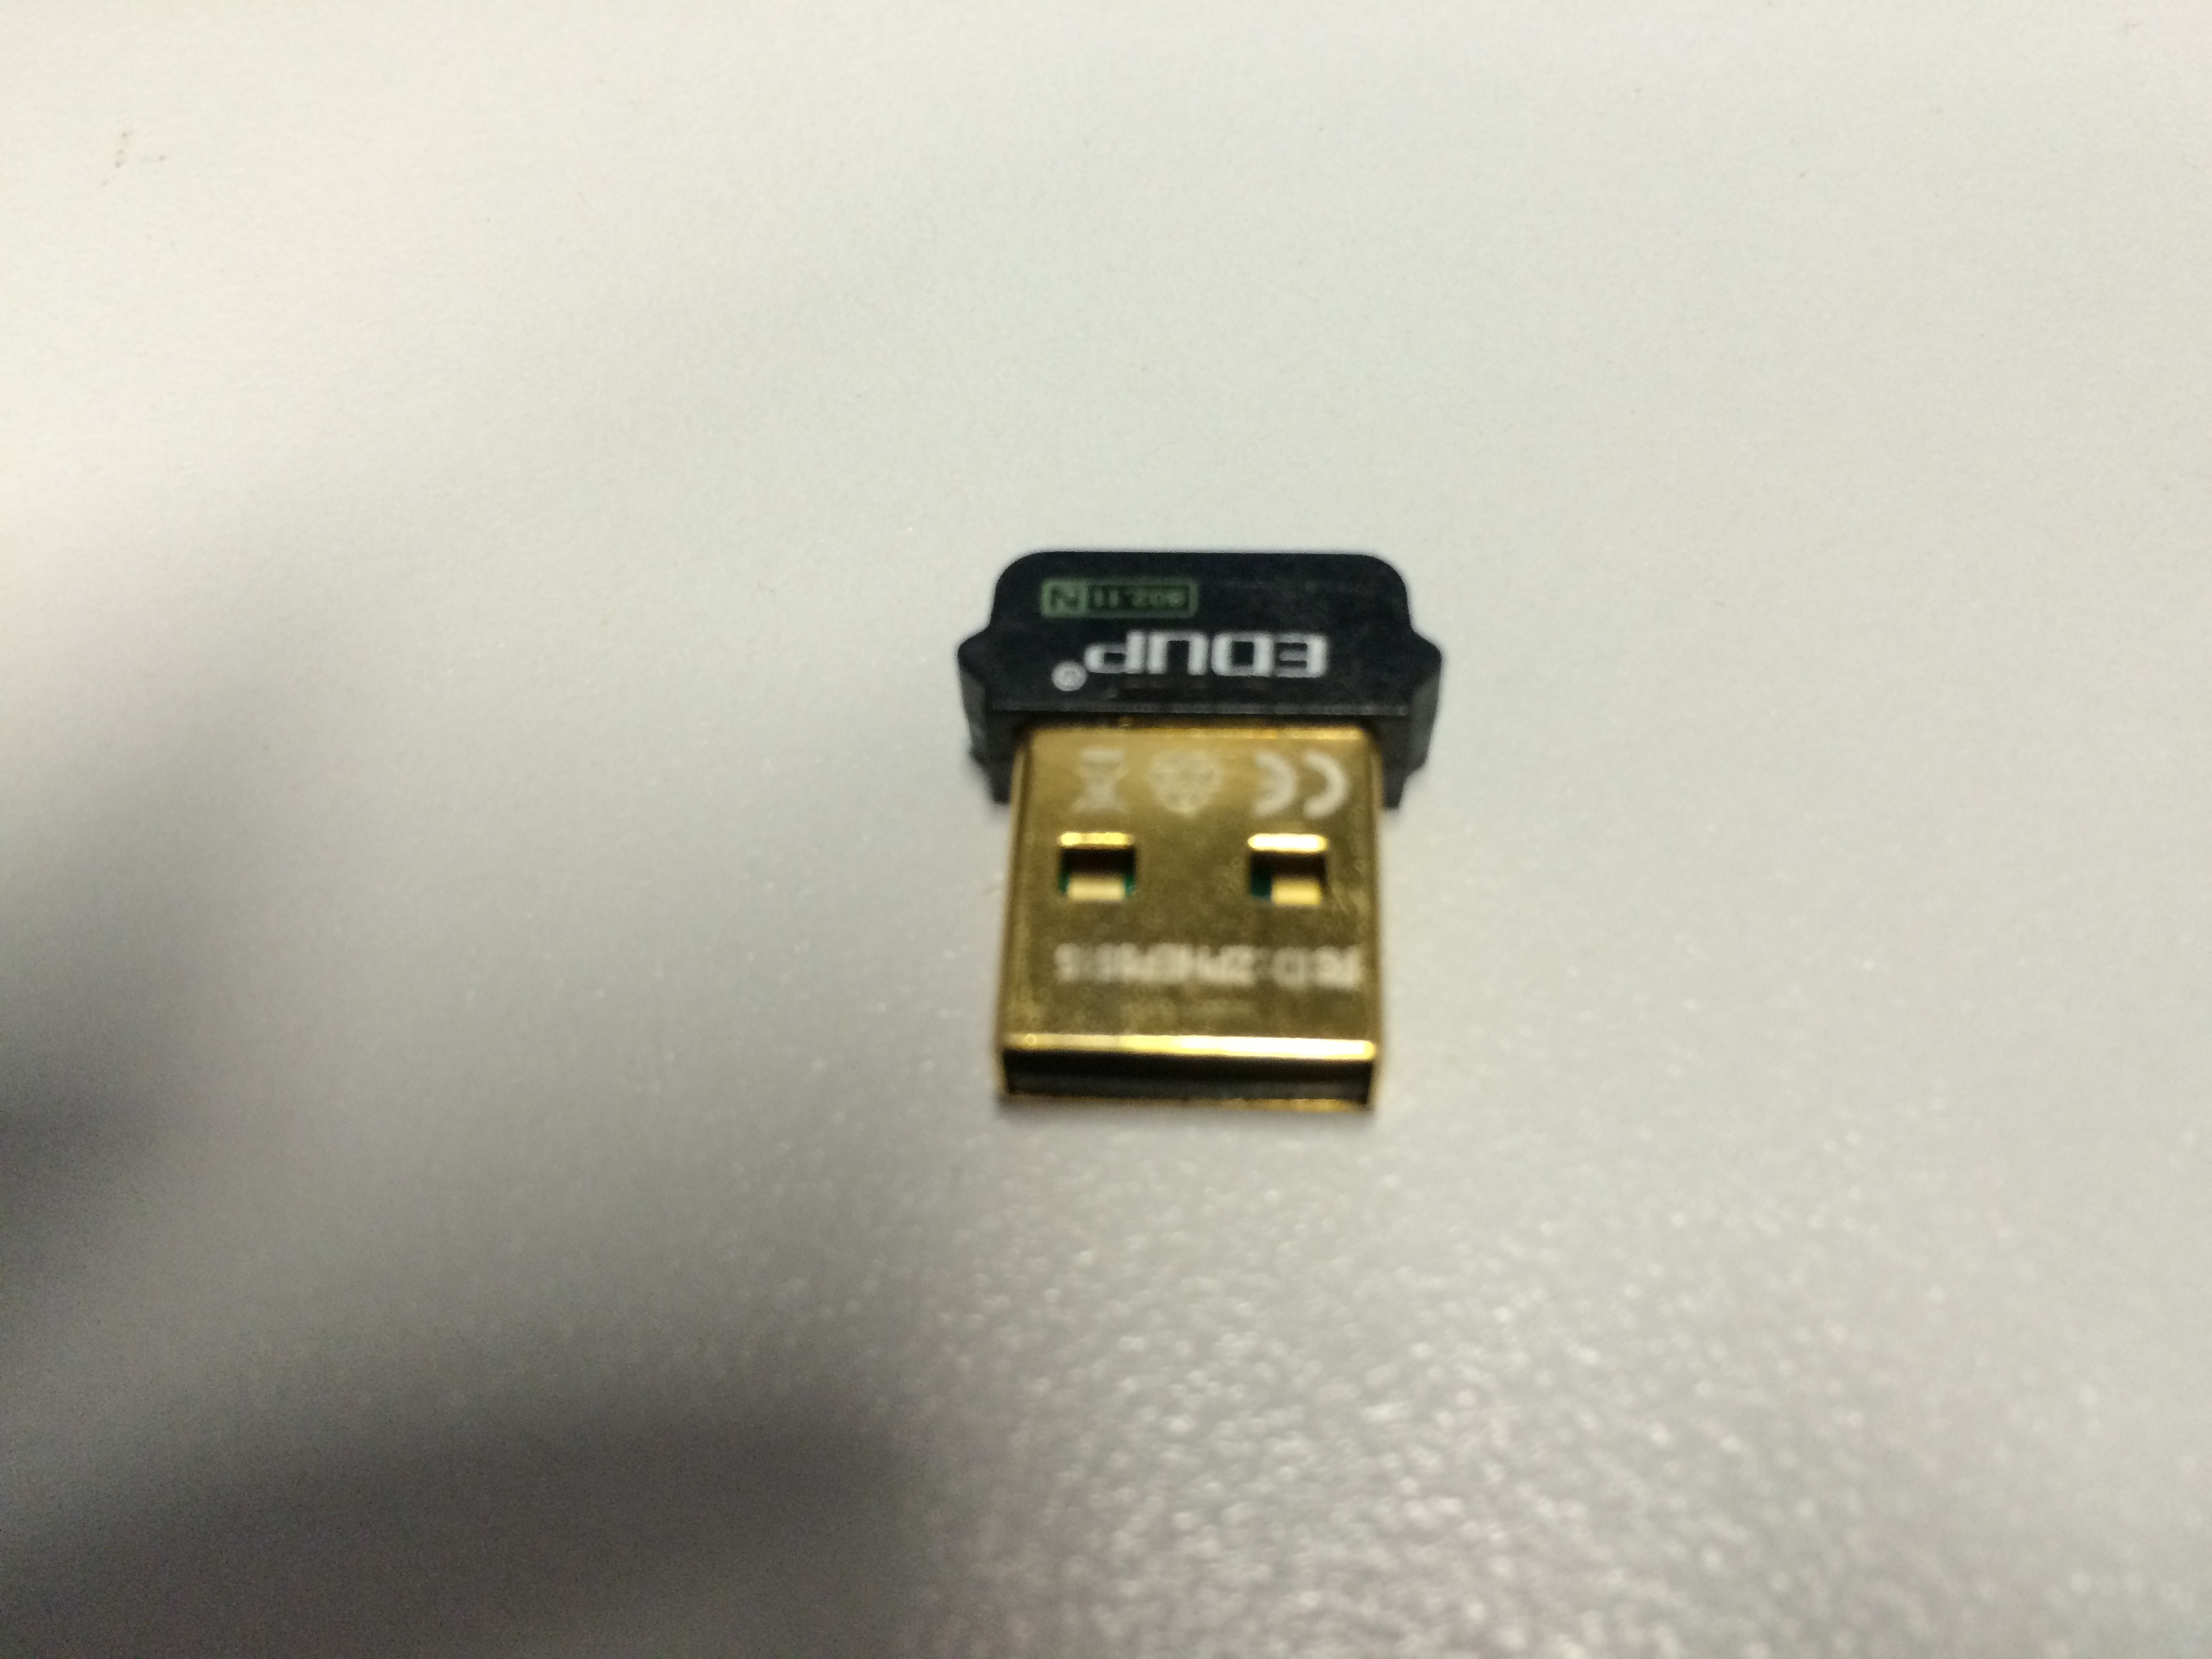
\includegraphics[width=2in]{./figs/wifiadapter.JPG}
       \label{wifiadapter.JPG}
     }
    \subfigure[Usb Hub.]{
       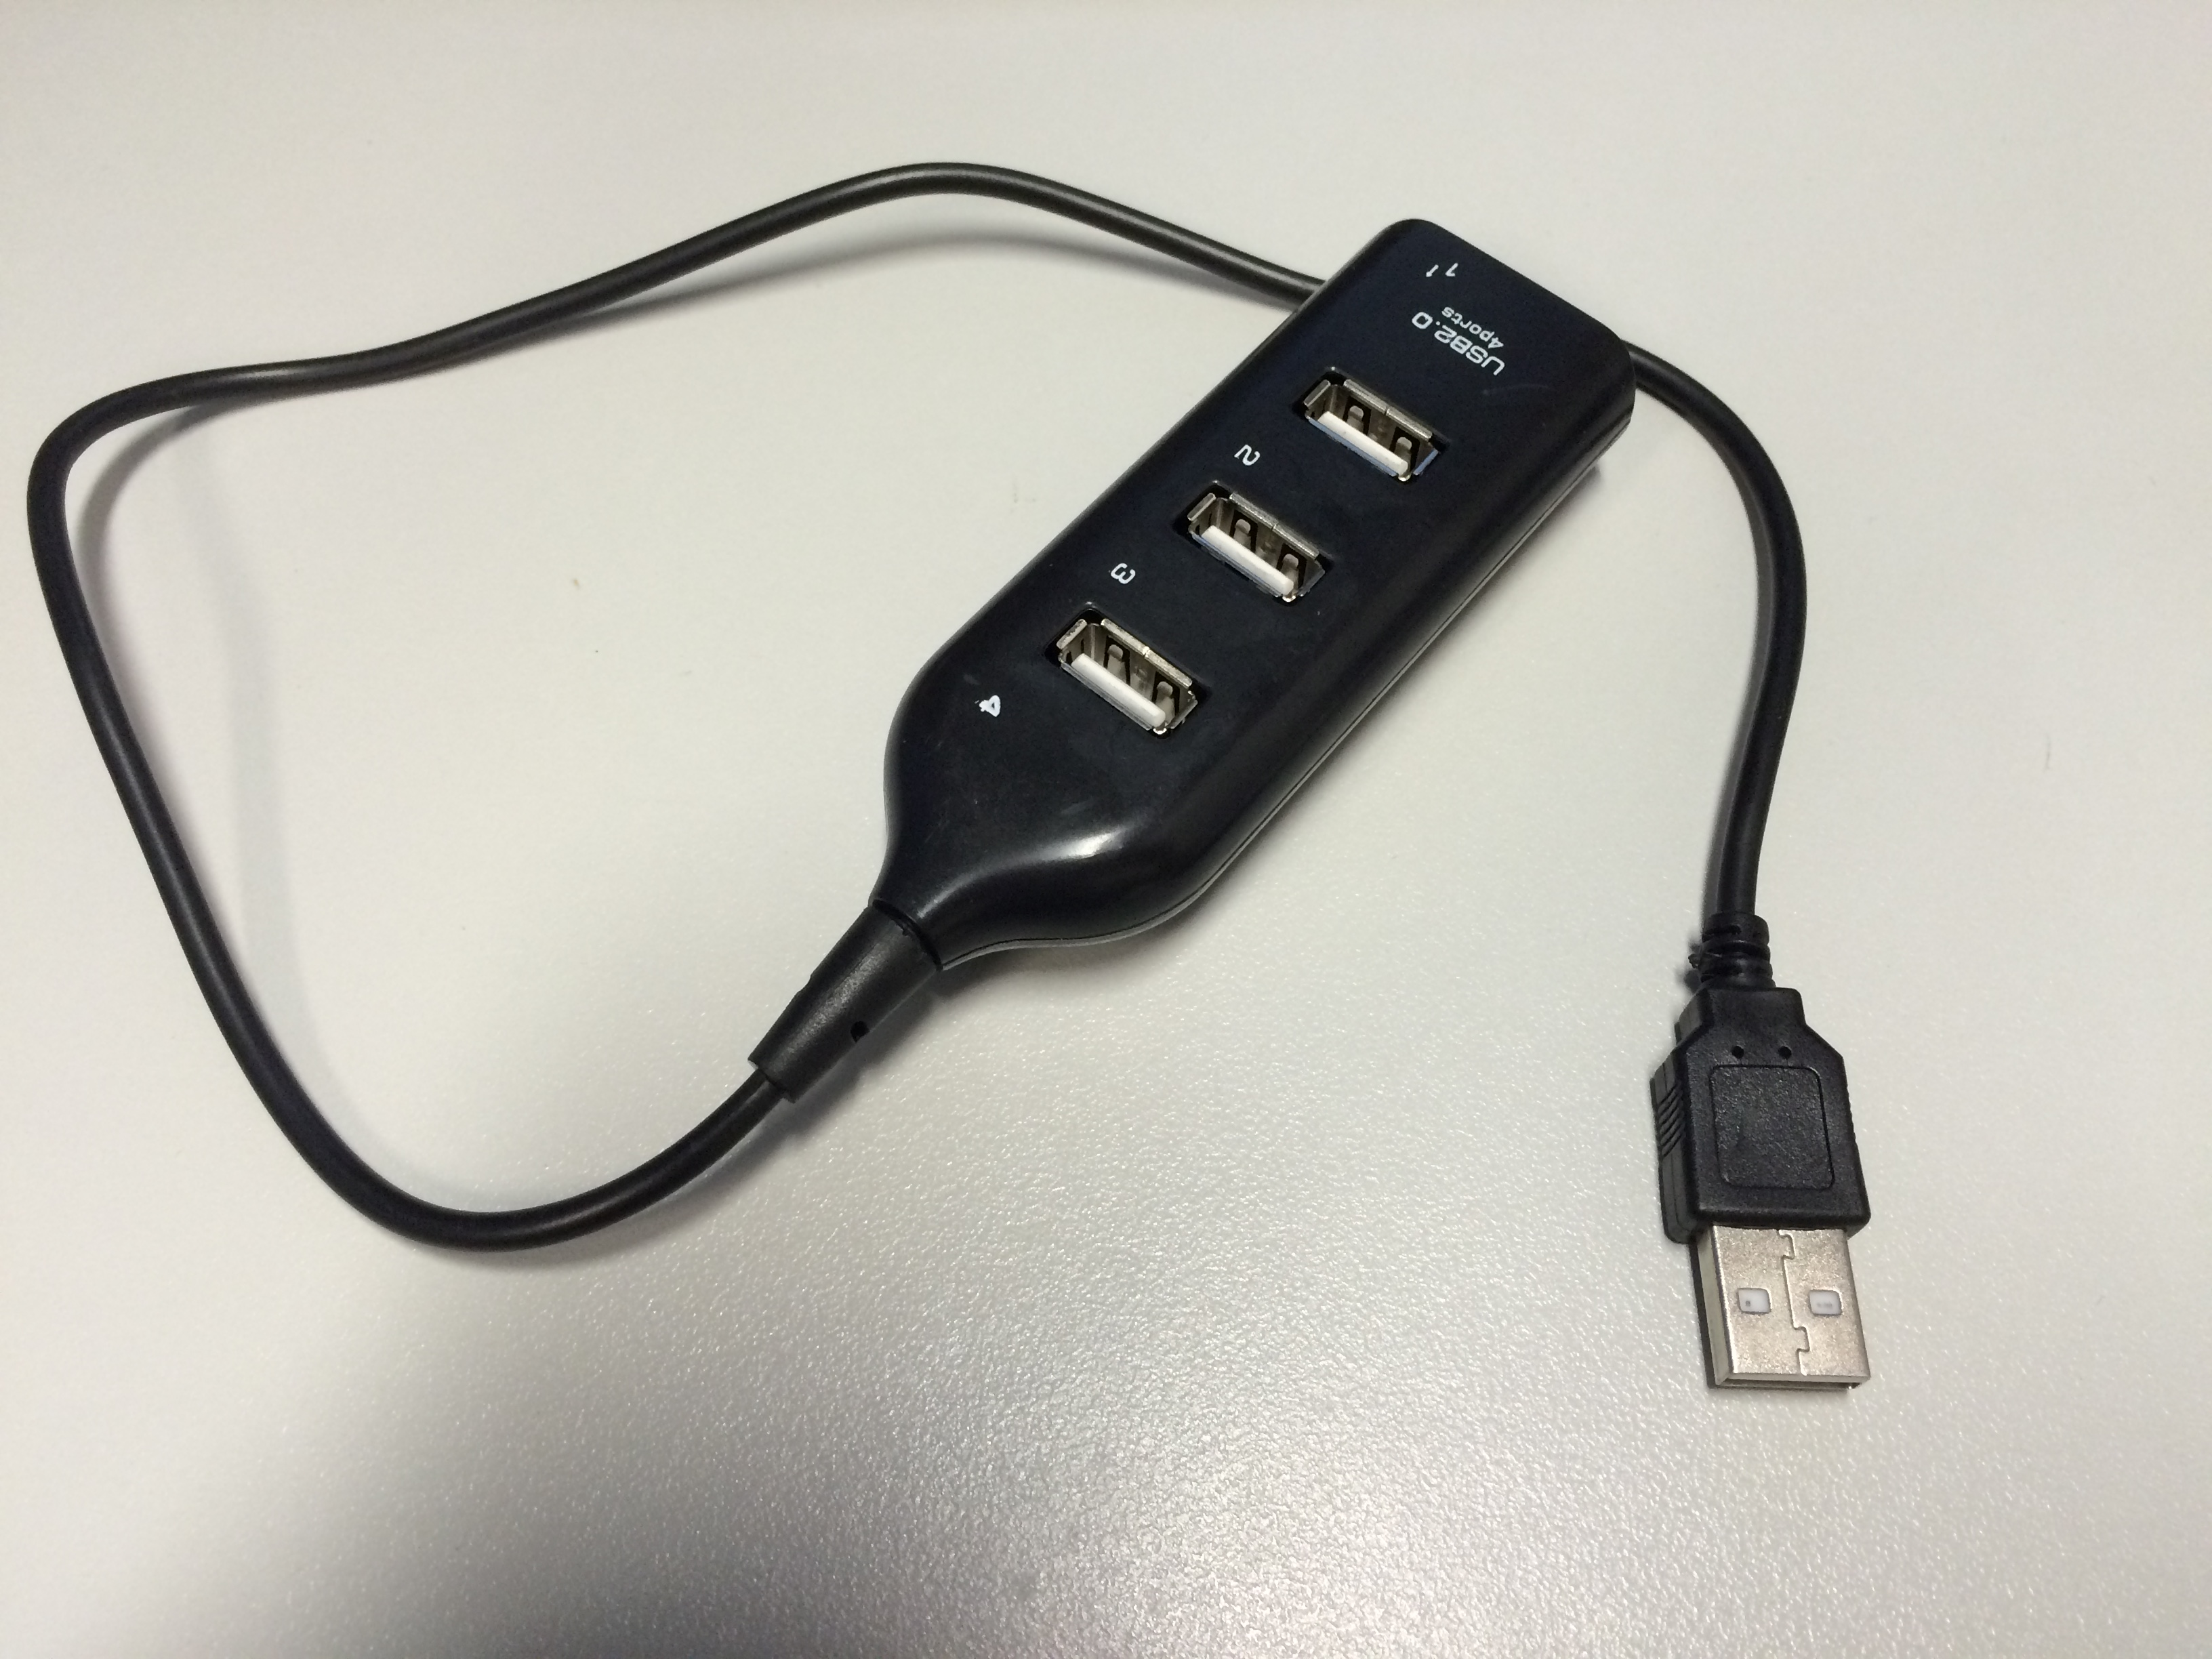
\includegraphics[width=2in]{./figs/usbhub.JPG}
       \label{usbhub.JPG}
     }
     \subfigure[MiniUSB Cable.]{
       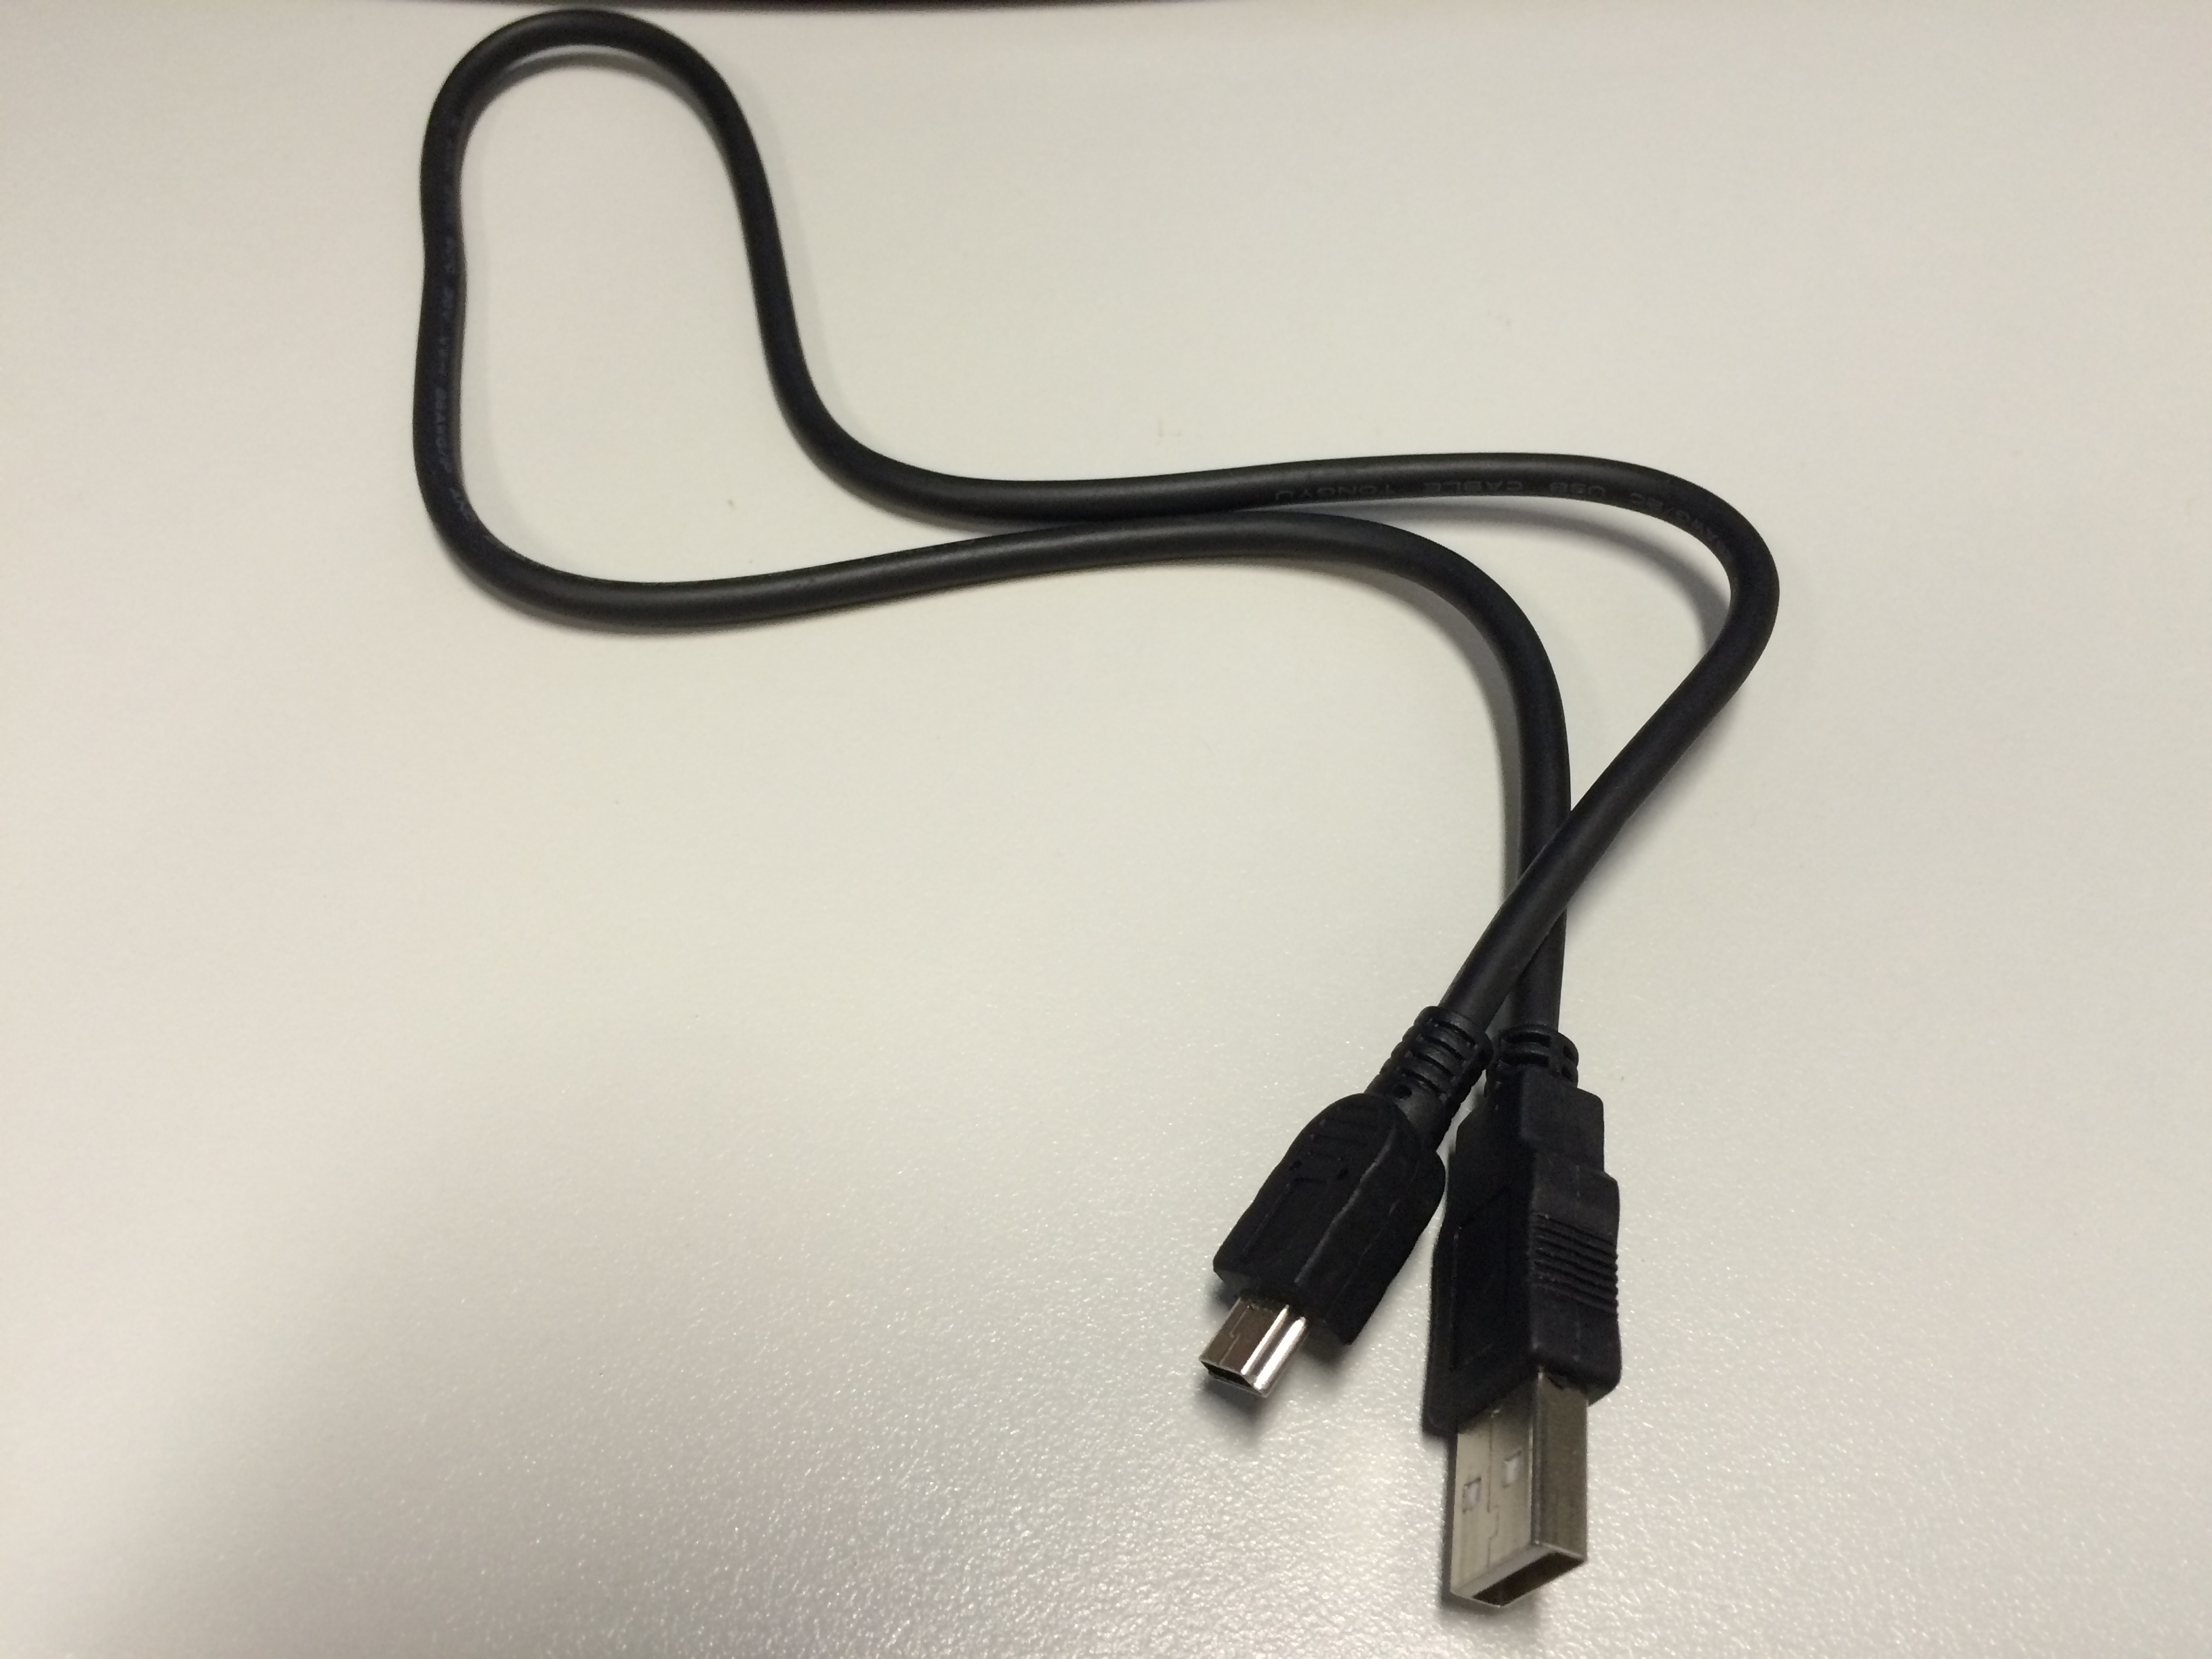
\includegraphics[width=2in]{./figs/miniusbcable.JPG}
       \label{miniusbcable.JPG}
     }
     \caption{Essential components for WiFi connection.}
     \label{WiFi}
     \end{figure}


To establish SSH connection, we must log on BBB via SSH protocol and this could be done with the help of SSH tool. In fact, there are a variety of SSH GUI tools available for Windows. In this report, we take the Secure Shell Client available on \textcolor{blue}{\textit{\url{http://mepopedia.com/forum/file.php?793,file=1103,filename=SSHSecureShellClient-3.2.9.exe,download=1}}}. Because of the integration of $scp$ command, this tool allows us to transfer files between the host PC and the BBB freely.

When the wireless network adapter is plug into BBB and BBB itself is also connected to one USB port on our host PC, we open the Secure Shell Client and start a SSH connection from PC to BBB as shown in Fig.\ref{ssh}. Remember the default Ethernet IP address for BBB is 192.168.7.2 and the default user account is `ubuntu' with password "temppwd".

Finally, we configure the WiFi setup by adding the following commands in the network configuration file located at /ect/network/interfaces:
\begin{lstlisting}[language={bash}]
#WiFi Example
auth wlan0
iface wlan0 inet dhcp
#WPA Enterprise setup
wpa-driver wext
wpa-ssid Universities WiFi
wpa-ap-scan 1
wpa-proto RSN
wpa-pairwise CCMP TKIP
wpa-group CCMP TKIP
wpa-eap PEAP
wpa-key-mgmt WPA-EAP
wpa-identity *yourEID*@my.cityu.edu.hk
wpa-password *yourPASSWORD*
\end{lstlisting}
The idea of this setup is to connect to CityU Campus WiFi network --- "Universities WiFi" with the student EID and password.

To make the modifications into effect, we type in the following command from Secure Shell Client to restart the wirless adapter:
\begin{lstlisting}[language={bash}]
ifconfig wlan0 down && ifconfig wlan0 up
\end{lstlisting}
By typing following command, the function of WiFi connection can be verified:
\begin{lstlisting}[language={bash}]
ping www.google.com.hk
\end{lstlisting}
Fig.\ref{ping} shows that the network setup is correct with all 4 transmitted packets getting received.





% % % % % % % % % % % % % % % % % % % % % % % % % % % % % % % % %
% % % % % % % % % % % % % % % % % % % % % % % % % % % % % % % % %	
\section{Conclusions}\label{Con}
In this project, we use BBB and embedded ARM-Linux as the hardware and software development tools, respectively. Implementing a series of functions including: Web server and SQL server setup and configuration; webpage based LED Test, Image/Video Capture and Face Detection; and MySQL based data storage functionality.

% % % % % % % % % % % % % % % % % % % % % % % % % % % % % % % % %
% % % % % % % % % % % % % % % % % % % % % % % % % % % % % % % % %

\bibliographystyle{plain}
\bibliography{bibfile}
\clearpage


\end{document}


